\documentclass{bhamthesis}
\title{Deep Three Match: Solving the game of three match with a learned evaluation function}
\author{Thomas Brereton}
\date{August 2017}  %% Version 2009/12/26

\usepackage{amsthm}
\usepackage{amssymb}
\usepackage{graphicx}


\newtheorem*{thm}{Theorem}

\theoremstyle{definition}
\newtheorem*{defn}{Definition}

\newcommand{\mar}[1]{\marginpar{\raggedright#1}}
\newcommand{\clsname}{\textsf{bhamthesis}}
\newcommand{\bktitle}[1]{\textit{#1}}
\newcommand{\ZF}{\mathrm{ZF}}
\newcommand{\IN}{\mathbb{N}}

\makeatletter
\newcommand{\makecrestcover}{%
\begin{titlepage}
\centering\singlespacing
\vspace*{1cm}
{\huge\bfseries University of Birmingham\par}
\vspace*{2cm}

\includegraphics[width=.3\textwidth]{media/img/crest}\par
\vspace*{\stretch{1}}
{\Huge\bfseries
\@author\par
\vspace{1cm}
\@title\par}
\vspace*{\stretch{1}}
{\Large\@date\par}
\end{titlepage}
}
\makeatother

\prefixappendix

\begin{document}
\frontmatter

%% Optional/alternative cover with crest
%\makecrestcover
\maketitle

%\tableofcontents


\mainmatter
\chapter{Proposal}
\section{Introduction}
In this thesis I will build an artificial intelligent (A.I.) agent which will play and solve the game of three match (think Candy Crush or Bejewelled).

The agent will be composed of a Monte Carlo tree search program, a neural network for the evaluation function, and a neural network for the policy. I will be focussing on the evaluation function and I aim to learn the features of the function using an auto-encoder, then train a neural network which uses these features that can evaluate the game state. I am collaborating with Elliott Davies who will design the policy, and we will both work together to implement the Monte Carlo search.

\section{Motivation}
I am interested in producing a similar program to that of AlphaGo, however, we will apply it to the game of Three Match, not Go. In Three Match the aim of the game is to match three pieces of the same type to break `ice' underneath and uncover all the `medals' (refer Figure \ref{f.gemisland}). Three Match comes with its own challenges, namely the highly random nature of which type of piece appears on the board. If three cells on the board need to be filled, the program must already consider 20 different potential states. This in combination with chain reactions of matches, leads to a tremendous branching factor and an enormous search space. 

In recent research most A.I. agents still use an evaluation function with hand-selected features, such is the case for AlphaGo. In this thesis we aim to use an auto-encoder and another neural network to learn the features of the function and then determine the optimal weights for the features. This will result in a evaluation function that is learned end-to-end by the program. Learning the entire evaluation function and the stochastic nature of the game make for a challenging project and I am interested to see if the agent can make successful short and long term tactical decisions.

\begin{figure}
\begin{center}
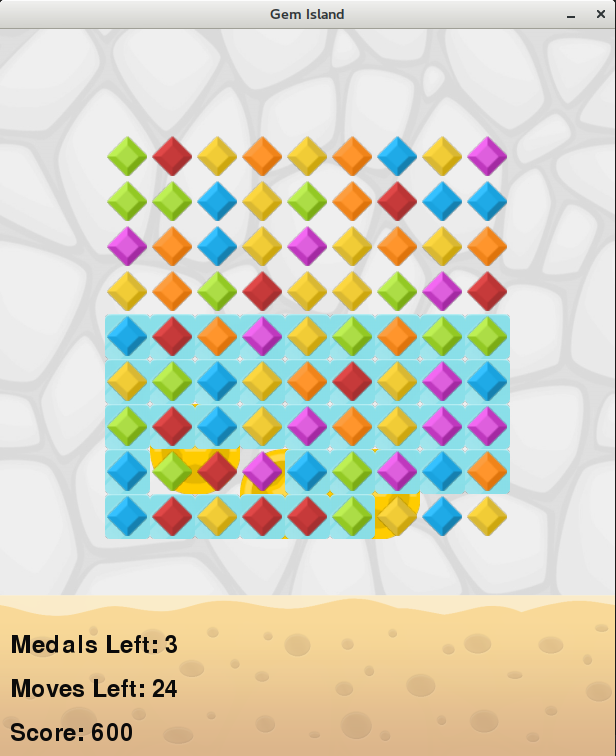
\includegraphics[scale=.3]{media/img/gem_island.png} 
\caption{The authors version of Three Match: Gem Island}
\label{f.gemisland}
\end{center}
\end{figure}



\section{Plan}

In this section I outline the work required to complete this thesis. Each table represents a task, which is broken down into sub-tasks in the description section. A Gantt chart is also included at the end for a graphical view of the project time line.

\begin{table}[]
\centering
\resizebox{\textwidth}{!}{%
\begin{tabular}{|l|l|}
\hline
Task         & 1. Complete game                                                                                                                                                                                                                                                                                                        \\ \hline
Due          & 2017/06/13                                                                                                                                                                                                                                                                                                              \\ \hline
Leader       & TB                                                                                                                                                                                                                                                                                                                      \\ \hline
Collaborator & ED                                                                                                                                                                                                                                                                                                                      \\ \hline
Objectives   & To build a challenging game for an AI agent to solve.                                                                                                                                                                                                                                                                   \\ \hline
Description  & \begin{tabular}[c]{@{}l@{}}1.1 Make a simple game for proof of concept\\ 1.2 Implement matches for gems\\ 1.3 Implement removable ice\\ 1.4 Implement 'gravity' to pull down gems\\ 1.5 Implement animations\\ 1.6 Implement scoring system\\ 1.7 Implement bonus gems\\ 1.8 Implement combination scoring\end{tabular} \\ \hline
Milestones   & \begin{tabular}[c]{@{}l@{}}1.1 Making a simple game\\ 1.6 A fully working game without bonuses\end{tabular}                                                                                                                                                                                                             \\ \hline
Deliverable  & A complete game for the AI to solve                                                                                                                                                                                                                                                                                     \\ \hline
\end{tabular}%
}
\end{table}

\begin{table}[]
\centering
\resizebox{\textwidth}{!}{%
\begin{tabular}{|l|l|}
\hline
Task         & 2. Set up game for AI                                                                                                                                             \\ \hline
Due          & 19/6/2017                                                                                                                                                         \\ \hline
Leader       & TB                                                                                                                                                                \\ \hline
Collaborator & ED                                                                                                                                                                \\ \hline
Objectives   & To get the game in a state for the AI to control.                                                                                                                 \\ \hline
Description  & \begin{tabular}[c]{@{}l@{}}2.1 Design the game state representation\\ 2.2 Implement methods to get game state\\ 2.3 Implement methods for AI to call\end{tabular} \\ \hline
Milestones   & -                                                                                                                                                                 \\ \hline
Deliverable  & A game designed so that an AI can control it.                                                                                                                     \\ \hline
\end{tabular}%
}
\end{table}

\begin{table}[]
\centering
\resizebox{\textwidth}{!}{%
\begin{tabular}{|l|l|}
\hline
Task         & 3. Build naive AI version 1                                                                                                                            \\ \hline
Due          & 22/6/2017                                                                                                                                              \\ \hline
Leader       & TB                                                                                                                                                     \\ \hline
Collaborator & ED                                                                                                                                                     \\ \hline
Objectives   & Proof of concept for getting an AI to control the game.                                                                                                 \\ \hline
Description  & \begin{tabular}[c]{@{}l@{}}3.1 Implement random policy/move selection\\ 3.2 Connect AI to game\\ 3.3 Collate training data from version 1\end{tabular} \\ \hline
Milestones   & -                                                                                                                                                      \\ \hline
Deliverable  & A working AI which can control the game.                                                                                                               \\ \hline
\end{tabular}%
}
\end{table}


\begin{table}[]
\centering
\resizebox{\textwidth}{!}{%
\begin{tabular}{|l|l|}
\hline
Task         & 4. Build naive AI version 2                                                                                                                                           \\ \hline
Due          & 28/6/2017                                                                                                                                                              \\ \hline
Leader       & TB                                                                                                                                                                     \\ \hline
Collaborator & ED                                                                                                                                                                     \\ \hline
Objectives   & Proof of concept for using MCTS, evaluation function, and a policy                                                                                                     \\ \hline
Description  & \begin{tabular}[c]{@{}l@{}}4.1 Design sarch, policy, and evaluation function (s, p, e)\\ 4.2 Implement s, p, e\\ 4.3 Collate training data from version 2\end{tabular} \\ \hline
Milestones   & -                                                                                                                                                                      \\ \hline
Deliverable  & A naive version of the final design of the AI.                                                                                                                         \\ \hline
\end{tabular}%
}
\end{table}

\begin{table}[]
\centering
\resizebox{\textwidth}{!}{%
\begin{tabular}{|l|l|}
\hline
Task         & 5. Gather and collate training data                                                                                                                     \\ \hline
Due          & 27/6/2017                                                                                                                                               \\ \hline
Leader       & TB                                                                                                                                                      \\ \hline
Collaborator & ED                                                                                                                                                      \\ \hline
Objectives   & To obtain the required training data for the neural networks.                                                                                           \\ \hline
Description  & \begin{tabular}[c]{@{}l@{}}5.1 Set up game to output state to file\\ 5.2 Set up game to distribute to users\\ 5.3 Distrubute game to users\end{tabular} \\ \hline
Milestones   & -                                                                                                                                                       \\ \hline
Deliverable  & \begin{tabular}[c]{@{}l@{}}Game to distribute - 22/06/17\\ Collated training data 27/07/17\end{tabular}                                                 \\ \hline
\end{tabular}%
}
\end{table}

\begin{table}[]
\centering
\resizebox{\textwidth}{!}{%
\begin{tabular}{|l|l|}
\hline
Task         & 6. Build neural network 1 (NN1) with hand selected features.                                               \\ \hline
Due          & 4/7/2017                                                                                                   \\ \hline
Leader       & TB                                                                                                         \\ \hline
Collaborator &                                                                                                            \\ \hline
Objectives   & To build a NN which evaluates the game state                                                               \\ \hline
Description  & \begin{tabular}[c]{@{}l@{}}6.1 Design and build NN1\\ 6.2 Train NN1\\ 6.3 Connect NN1 to game\end{tabular} \\ \hline
Milestones   & -                                                                                                          \\ \hline
Deliverable  & AI agent with working NN                                                                                   \\ \hline
\end{tabular}%
}
\end{table}

\begin{table}[]
\centering
\resizebox{\textwidth}{!}{%
\begin{tabular}{|l|l|}
\hline
Task         & 7. Build neural network 2 (NN2) with learned evaluation function.                                                                                         \\ \hline
Due          & 14/7/2017                                                                                                                                                 \\ \hline
Leader       & TB                                                                                                                                                        \\ \hline
Collaborator &                                                                                                                                                           \\ \hline
Objectives   & To build a NN which learns the function features and evaluates the game state.                                                                            \\ \hline
Description  & \begin{tabular}[c]{@{}l@{}}7.1 Design and build auto-encoder\\ 7.2 Build NN2 with learned features\\ 7.3 Train NN2\\ 7.4 Connect NN1 to game\end{tabular} \\ \hline
Milestones   & -                                                                                                                                                         \\ \hline
Deliverable  & AI agent with fully learned evaluation function.                                                                                                          \\ \hline
\end{tabular}%
}
\end{table}

\begin{table}[]
\centering
\resizebox{\textwidth}{!}{%
\begin{tabular}{|l|l|}
\hline
Task         & 8. Build Monte Carlo tree search program                                                                   \\ \hline
Due          & 21/7/2017                                                                                                  \\ \hline
Leader       & ED                                                                                                         \\ \hline
Collaborator & TB                                                                                                         \\ \hline
Objectives   & To build a tree search program to solve the game.                                                          \\ \hline
Description  & \begin{tabular}[c]{@{}l@{}}8.1 Build and design MCTS program\\ 8.2 Connect MCTS program to AI\end{tabular} \\ \hline
Milestones   & -                                                                                                          \\ \hline
Deliverable  & A working AI similar in design to AlphaGo                                                                  \\ \hline
\end{tabular}%
}
\end{table}

\begin{table}[]
\centering
\resizebox{\textwidth}{!}{%
\begin{tabular}{|l|l|}
\hline
Task         & 9. Write dissertation                                                                                                                                                                                                                                                                                                                                                                                \\ \hline
Due          & 13/8/2017                                                                                                                                                                                                                                                                                                                                                                                            \\ \hline
Leader       & ED                                                                                                                                                                                                                                                                                                                                                                                                   \\ \hline
Collaborator & TB                                                                                                                                                                                                                                                                                                                                                                                                   \\ \hline
Objectives   & To write a dissertation.                                                                                                                                                                                                                                                                                                                                                                             \\ \hline
Description  & \begin{tabular}[c]{@{}l@{}}9.1 Outline of dissertation 26/06/17\\ 9.2 Literature review 21/06/17\\ 9.3 Definition of problem 03/07/17\\ 9.4 Solution to problem 03/07/17\\ 9.5 Why is it novel 03/07/17\\ 9.6 Methodology for NN1 06/07/17\\ 9.7 Half draft 02/07/17\\ 9.8 Full methodology including NN2, search, policy 24/07/17\\ 9.9 Full draft 31/07/17\\ 9.10 Final copy 13/08/17\end{tabular} \\ \hline
Milestones   & -                                                                                                                                                                                                                                                                                                                                                                                                    \\ \hline
Deliverable  & \begin{tabular}[c]{@{}l@{}}Half draft 02/07/17\\ Full draft 31/07/17\end{tabular}                                                                                                                                                                                                                                                                                                                    \\ \hline
\end{tabular}%
}
\end{table}


\end{document}